\section{Solar Collectors }\label{solar-collectors}

Solar collectors are devices that convert solar energy into thermal energy by raising the temperature of a circulating heat transfer fluid.~ The fluid can then be used to heat water for domestic hot water usage or space heating.~ Flat-plate solar collectors using water as the heat transfer fluid, Integral-Collector Storage solar collectors using water and unglazed transpired solar collectors using air are currently the only types of collector available in EnergyPlus.

\subsection{Flat-Plate Solar Collectors}\label{flat-plate-solar-collectors}

The input object SolarCollector:FlatPlate:Water provides a model for flat-plate solar collectors that are the most common type of collector.~ Standards have been established by ASHRAE for the performance testing of these collectors (ASHRAE 1989; 1991) and the Solar Rating and Certification Corporation (SRCC) publishes a directory of commercially available collectors in North America (SRCC 2003).

The EnergyPlus model is based on the equations found in the ASHRAE standards and Duffie and Beckman (1991).~ This model applies to glazed and unglazed flat-plate collectors, as well as banks of tubular, i.e.~evacuated tube, collectors.

\subsubsection{Solar and Shading Calculations}\label{solar-and-shading-calculations-000}

The solar collector object uses a standard EnergyPlus surface in order to take advantage of the detailed solar and shading calculations.~ Solar radiation incident on the surface includes beam and diffuse radiation, as well as radiation reflected from the ground and adjacent surfaces.~ Shading of the collector by other surfaces, such as nearby buildings or trees, is also taken into account.~ Likewise, the collector surface can shade other surfaces, for example, reducing the incident radiation on the roof beneath it.

\subsubsection{Thermal Performance}\label{thermal-performance}

The thermal efficiency of a collector is defined as the ratio of the useful heat gain of the collector fluid versus the total incident solar radiation on the gross surface area of the collector.

\begin{equation}
\eta  = \frac{{(q/A)}}{{{I_{solar}}}}
\label{eq:SolarCollectorEta}
\end{equation}

where:

\emph{q} is the useful heat gain

\emph{A} is the gross area of the collector

\(I_{solar}\) is the total incident solar radiation.

Notice that the efficiency h is only defined for I\(_{solar}\) \textgreater{} 0.

An energy balance on a solar collector with double glazing shows relationships between the glazing properties, absorber plate properties, and environmental conditions.

\begin{equation}
\frac{q}{A} = {I_{solar}}{\tau_{g1}}{\tau_{g2}}{\alpha_{abs}} - \frac{{T_{abs}^4 - T_{g2}^4}}{{{R_{rad}}}} - \frac{{{T_{abs}} - {T_{g2}}}}{{{R_{conv}}}} - \frac{{{T_{abs}} - {T_{air}}}}{{{R_{cond}}}}
\end{equation}

where:

\(\tau_{g1}\) is the transmittance of the first glazing layer

\(\tau_{g2}\) is the transmittance of the second glazing layer

\(\alpha_{abs}\) is the absorptance of the absorber plate

\(R_{rad}\) is the radiative resistance from absorber to inside glazing

\(R_{conv}\) is the convective resistance from absorber to inside glazing

\(R_{cond}\) is the conductive resistance from absorber to outdoor air through the insulation

\(T_{abs}\) is the temperature of the absorber plate

\(T_{g2}\) is the temperature of the inside glazing

\(T_{air}\) is the temperature of the outdoor air.

The equation above can be approximated with a simpler formulation as:

\begin{equation}
\frac{q}{A} = {F_R}\left[ {{I_{solar}}(\tau \alpha ) - {U_L}({T_{in}} - {T_{air}})} \right]
\label{eq:SolarCollectorqOverA697}
\end{equation}

where:

\(F_{R}\) is an empirically determined correction factor

(\(\tau \alpha\)) is the product of all transmittance and absorptance terms

\(U_{L}\) is the overall heat loss coefficient combining radiation, convection, and conduction terms

\(T_{in}\) is the inlet temperature of the working fluid.

Substituting this into Equation~\ref{eq:SolarCollectorEta},

\begin{equation}
\eta  = {F_R}(\tau \alpha ) - {F_R}{U_L}\frac{{({T_{in}} - {T_{air}})}}{{{I_{solar}}}}
\label{eq:SolarCollectorEta698}
\end{equation}

A linear correlation can be constructed by treating F\(_{R}\)(\(\tau \alpha\)) and -F\(_{R}\)U\(_{L}\) as characteristic constants of the solar collector:

\begin{equation}
\eta  = {c_0} + {c_1}\frac{{\left( {{T_{in}} - {T_{air}}} \right)}}{{{I_{solar}}}}
\end{equation}

Similarly, a quadratic correlation can be constructed using the form:

\begin{equation}
\eta  = {c_0} + {c_1}\frac{{\left( {{T_{in}} - {T_{air}}} \right)}}{{{I_{solar}}}} + {c_2}\frac{{{{\left( {{T_{in}} - {T_{air}}} \right)}^2}}}{{{I_{solar}}}}
\end{equation}

Both first- and second-order efficiency equation coefficients are listed in the \emph{Directory of SRCC Certified Solar Collector Ratings}.

\subsubsection{Incident Angle Modifiers}\label{incident-angle-modifiers}

As with regular windows the transmittance of the collector glazing varies with the incidence angle of radiation.~ Usually the transmittance is highest when the incident radiation is normal to the glazing surface.~ Test conditions determine the efficiency coefficients for normal incidence.~ For off-normal angles, the transmittance of the glazing is modified by an \emph{incident angle modifier} coefficient.

\begin{equation}
{K_{\tau \alpha }} = \frac{{\left( {\tau \alpha } \right)}}{{{{\left( {\tau \alpha } \right)}_n}}}
\end{equation}

Additional testing determines the incident angle modifier as a function of incident angle \(\theta\).~ This relationship can be fit to a first-order, linear correlation:

\begin{equation}
{K_{\tau \alpha }} = 1 + {b_0}\left( {\frac{1}{{\cos \theta }} - 1} \right)
\end{equation}

or a second-order, quadratic correlation:

\begin{equation}
{K_{\tau \alpha }} = 1 + {b_0}\left( {\frac{1}{{\cos \theta }} - 1} \right) + {b_1}{\left( {\frac{1}{{\cos \theta }} - 1} \right)^2}
\end{equation}

The incident angle modifier coefficients \emph{b\(_{0}\)} and \emph{b\(_{1}\)} are usually negative, although some collectors have a positive value for \emph{b\(_{0}\)}.~ Both first- and second-order incident angle modifier equation coefficients are listed in the \emph{Directory of SRCC Certified Solar Collector Ratings}.

The SRCC incident angle modifier equation coefficients are only valid for incident angles of 60 degrees or less.~ Because these curves can be valid yet behave poorly for angles greater than 60 degree, the EnergyPlus model cuts off collector gains for incident angles greater than 60 degrees.

For flat-plate collectors, the incident angle modifier is generally symmetrical.~ However, for tubular collectors the incident angle modifier is different depending on whether the incident angle is parallel or perpendicular to the tubes.~ These are called bi-axial modifiers.~ Some special flat-plate collectors may also exhibit this asymmetry.~ The current model cannot yet handle two sets of incident angle modifiers.~ In the meantime it is recommended that tubular collectors be approximated with caution using either the parallel or perpendicular correlation.

Incident angle modifiers are calculated separately for sun, sky, and ground radiation.~ The net incident angle modifier for all incident radiation is calculated by weighting each component by the corresponding modifier.

\begin{equation}
{K_{\tau \alpha ,net}} = \frac{{{I_{beam}}{K_{\tau \alpha ,beam}} + {I_{sky}}{K_{\tau \alpha ,sky}} + {I_{gnd}}{K_{\tau \alpha ,gnd}}}}{{{I_{beam}} + {I_{sky}} + {I_{gnd}}}}
\end{equation}

For sky and ground radiation the incident angle is approximated using Brandemuehl and Beckman's equations:

\begin{equation}
{\theta_{sky}} = 59.68 - 0.1388\phi  + 0.001497{\phi ^2}
\end{equation}

\begin{equation}
{\theta_{ground}} = 90.0 - 0.5788\phi  + 0.002693{\phi ^2}
\end{equation}

where \(\phi\) is the surface tilt in degrees.

The net incident angle modifier is then inserted into the useful heat gain Equation~\ref{eq:SolarCollectorqOverA697}:

\begin{equation}
\frac{q}{A} = {F_R}\left[ {{I_{solar}}{K_{\tau \alpha ,net}}{{(\tau \alpha )}_n} - {U_L}({T_{in}} - {T_{air}})} \right]
\label{eq:SolarCollectorqOverA707}
\end{equation}

Equation~\ref{eq:SolarCollectorEta698} is also modified accordingly.

\begin{equation}
\eta  = {F_R}{K_{\tau \alpha ,net}}{(\tau \alpha )_n} - {F_R}{U_L}\frac{{({T_{in}} - {T_{air}})}}{{{I_{solar}}}}
\end{equation}

\subsubsection{Outlet Temperature}\label{outlet-temperature}

Outlet temperature is calculated using the useful heat gain q as determined by Equation~\ref{eq:SolarCollectorqOverA707}, the inlet fluid temperature T\(_{in}\), and the mass flow rate available from the plant simulation:

\begin{equation}
\frac{q}{A} = \dot m{c_p}({T_{out}} - {T_{in}})
\end{equation}

where:

\(\dot m\) is the fluid mass flow rate through the collector

\(c_{p}\) is the specific heat of the working fluid.

Solving for T\(_{out}\),

\begin{equation}
{T_{out}} = {T_{in}} + \frac{q}{{\dot m{c_p}A}}
\end{equation}

If there is no flow through the collector, T\(_{out}\) is the stagnation temperature of the fluid.~ This is calculated by setting the left side of Equation~\ref{eq:SolarCollectorqOverA707} to zero and solving for T\(_{in}\) (which also equals T\(_{out}\) for the no flow case).

\subsubsection{References}\label{references-042}

ASHRAE.~ 1989.~ ASHRAE Standard 96-1980 (RA 89):~ Methods of Testing to Determine the Thermal Performance of Unglazed Flat-Plate Liquid-Type Solar Collectors.~ Atlanta: American Society of Heating, Refrigerating and Air-Conditioning Engineers, Inc.

ASHRAE.~ 1991.~ ASHRAE Standard 93-1986 (RA 91):~ Methods of Testing to Determine the Thermal Performance of Solar Collectors.~ Atlanta: American Society of Heating, Refrigerating and Air-Conditioning Engineers, Inc.

Duffie, J. A., and Beckman, W. A.~ 1991.~ Solar Engineering of Thermal Processes, Second Edition.~ New York:~ Wiley-Interscience.

Solar Rating and Certification Corporation.~ 2004.~ Directory of SRCC Certified Solar Collector Ratings, OG 100.~ Cocoa, Florida:~ Solar Rating and Certification Corporation.

\subsection{Integral-collector-storage (ICS) Solar Collector}\label{integral-collector-storage-ics-solar-collector}

Solar collectors with integral storage unit models use SolarCollector:IntegralCollectorStorage object, and the characteristics parameter inputs of this collector are provided by the SolarCollectorPerformance:IntegralCollectorStorage object. This model is based on detailed Energy Balance equations of solar collectors that integrates storage in it. This model has two options to represent the collector bottom outside boundary conditions: AmbientAir, and OtherSideConditionsModel. AmbientAir simply applies outside air temperature using combined convection and radiation conductance, and the OtherSideConditionsModel applies combined radiation and convection models that exiats in a naturally ventilated cavity to represent the collector bottom outside boundary condition. The later boundary condition accounts for the shading of the collector on the underlying surface, hence, the ICS collector can be assumed as an integral part of the building envelope. Schematic diagram of a rectangular ICS solar collector is shown in Figure~\ref{fig:schematic-diagram-of-rectangular-integrated} below:

\begin{figure}[hbtp] % fig 295
\centering
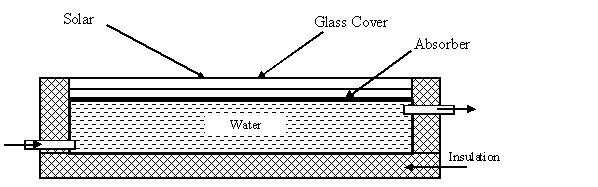
\includegraphics[width=0.9\textwidth, height=0.9\textheight, keepaspectratio=true]{media/image6502.png}
\caption{Schematic diagram of rectangular Integrated Collector Storage unit \protect \label{fig:schematic-diagram-of-rectangular-integrated}}
\end{figure}

\subsubsection{Solar and Shading Calculations}\label{solar-and-shading-calculations-1}

The solar collector object uses a standard EnergyPlus surface in order to take advantage of the detailed solar and shading calculations. Solar radiation incident on the surface includes beam and diffuse radiation, as well as radiation reflected from the ground and adjacent surfaces. Shading of the collector by other surfaces, such as nearby buildings or trees, is also taken into account. Likewise, the collector surface shades the roof surface beneath it, hence no direct solar radiation incident on the roof surface. The collector and the roof outside boundary conditions should be specified as OtherSideConditionModel to account for solar collector shading impact on the roof surface.

\subsubsection{Mathematical Model}\label{mathematical-model}

The integral-collector-storage (ICS) solar collector is represented using two transient energy balance equations shown below.~ These equations represent the energy balance equation for the absorber plate, and the water in the collector.

\begin{equation}
{m_p}{C_p}\frac{{d{T_p}}}{{dt}} = A \cdot \left[ {{{\left( {\tau \alpha } \right)}_e} \cdot {I_t} - {h_{pw}}\left( {{T_p} - {T_w}} \right) - {U_t}\left( {{T_p} - {T_a}} \right)} \right]
\end{equation}

\begin{equation}
{m_w}{C_w}\frac{{d{T_w}}}{{dt}} = A \cdot \left[ {{h_{pw}}\left( {{T_p} - {T_w}} \right) - {U_b}\left( {{T_w} - {T_{OSC}}} \right) - {U_s}\left( {{T_w} - {T_a}} \right)} \right] - {\dot m_w}{C_w}\left( {{T_w} - {T_{wi}}} \right)
\end{equation}

where:

\(m_{p} C_{p}\) is the thermal capacity of the absorber surface, J/\(^{\circ}\)C

\(A\) is the collector gross area, m\(^{2}\)

\({(\tau \alpha)}_{e}\) is the transmittance-absorptance product of the absorber plate and cover system

\(I_{t}\) is the total solar irradiation (W/m\(^{2}\))

\(h_{pw}\) is the convective heat transfer coefficient from absorber plate to water (W/m\(^2\)-K)

\(U_{t}\) is the overall heat loss coefficient from absorber to the ambient air (W/m\(^2\)-K)

\(T_{p}\) is the absorber plate average temperature (\(^{\circ}\)C)

\(T_{w}\) is the collector water average temperature (\(^{\circ}\)C)

\(T_{a}\) is the ambient air temperature (\(^{\circ}\)C)

\(m_{w} C_{pw}\) is the thermal capacity of the water mass in the collector (J/\(^{\circ}\)C)

\(U_{s}\) is the area-weighted conductance of the collector side insulation (W/m\(^{2}\)-K)

\(U_{b}\) is the conductance of the collector bottom insulation (W/m\(^{2}\)-K)

\(T_{osc}\) is the outside temperature of bottom insulation determined from the other side condition model (\(^{\circ}\)C)

\(T_{wi}\) is the entering makeup or mains water temperature (\(^{\circ}\)C)

\({\dot m_w}{C_w}\) is the water capacity flow through the collector (W/\(^{\circ}\)C).

The other side condition model boundary condition represented by the \emph{T\(_{osc}\)}, allows us to apply a realistic outside boundary condition for a collector mounted on a building roof.~ This also accounts for the shading impact of the collector on the under-laying surface (roof).~ On the other hand if ambient air boundary condition is specified, then the collector does not shade the underlying surface it is mounted on.

The two energy balance equation can be written as non-homogeneous first order DE with constant coefficients. The initial conditions for these equations are the absorber plate average temperature and the collector water average temperature at previous time steps.

\begin{equation}
\frac{{d{T_p}}}{{dt}} = {a_1}{T_p} + {a_2}{T_w} + {a_3}
\end{equation}

\begin{equation}
\frac{{d{T_w}}}{{dt}} = {b_1}{T_p} + {b_2}{T_w} + {b_3}
\end{equation}

\begin{equation}
{a_1} =  - \left( {A \cdot {h_{pw}} + A \cdot {U_t}} \right)/\left( {{m_p} \cdot {C_p}} \right)
\end{equation}

\begin{equation}
{a_2} = A \cdot {h_{pw}}{T_w}/\left( {{m_p} \cdot {C_p}} \right)
\end{equation}

\begin{equation}
{a_3} = A \cdot {\left( {\tau \alpha } \right)_e} \cdot {I_t} + A \cdot {U_t}{T_a}
\end{equation}

\begin{equation}
{b_1} = A \cdot {h_{pw}}{T_p}/\left( {{m_w} \cdot {C_w}} \right)
\end{equation}

\begin{equation}
{b_2} =  - \left( {A \cdot {h_{pw}} + A \cdot {U_b} + A \cdot {U_s} + {{\dot m}_w}{C_w}} \right)
\end{equation}

\begin{equation}
{{\rm{b}}_{\rm{3}}} = {\rm{ }}\left( {A \cdot {U_b}{T_{osc}} + A \cdot {U_s}{T_a} + {{\dot m}_w}{C_w}{T_{wi}}} \right)
\end{equation}

The two coupled first order differential equation are solved analytically.~ Auxiliary equation of the the coupled homogeneous differential equation is given by:

\begin{equation}
{\lambda ^2} - ({a_1} + {b_2}) + ({a_1}{b_2} - {a_2}{b_1}) = 0
\end{equation}

This auxiliary quadratic equation has always two distinct real roots (\(\lambda_{1}\) and \(\lambda_{2}\)) hence the solution of the homogeneous equation is exponential, and the general solutions of the differential equations are given by:

\begin{equation}
{T_p} =  {c_1}{e^{{\lambda_1}t}} + {c_2}{e^{{\lambda_2}t}} + A
\end{equation}

\begin{equation}
{T_w} =  {r_1}{c_1}{e^{{\lambda_1}t}} + {r_2}{c_2}{e^{{\lambda_2}t}} + B
\end{equation}

The constant terms \emph{A} and \emph{B} are the particular solution of the non-homogeneous differential equations, the coefficients of the exponential terms (\emph{c\(_{1}\)}, \emph{c\(_{2}\)}, \emph{r\(_{1}\)}, and \emph{r\(_{2}\)}) are determined from the initial conditions of the absorber and collector water temperatures (\emph{T\(_{p0}\)}, \emph{T\(_{w0}\)}) and are given by:

\begin{equation}
{r_1} =  ({\lambda_1} - {a_1})/{a_2};\quad {r_2} =  ({\lambda_2} - {a_1})/{a_2}
\end{equation}

\begin{equation}
A =  ( - {a_3}{b_2} + {b_3}{a_2})/({a_1}{b_2} - {b_1}{a_2});\quad B =  ( - {a_1}{b_3} + {b_1}{a_3})/({a_1}{b_2} - {b_1}{a_2})
\end{equation}

\begin{equation}
{c_1} =  ({r_2}{T_{p0}} - {T_{w0}} - {r_2}A + B)/({r_2} - {r_1});\quad {c_2} =  ({T_{w0}} - {r_1}{T_{p0}} + {r_1}A - B)/({r_2} - {r_1})
\end{equation}

\subsubsection{Thermal Network Model:}\label{thermal-network-model}

The thermal network model requires energy balance for each of the collector covers as well.~ The heat balance equation of the collector covers is assumed to obey steady state formulation by ignoring their thermal mass. The thermal-network representation of the ICS collector is shown in Figure~\ref{fig:thermal-network-diagram-for-ics-solar}. Also, the heat balance at each cover surface requires knowledge of the amount of solar fraction absorbed, which is determined from the ray tracing analysis. For the thermal network model shown above the overall top heat loss coefficient is determined from combination of the resistances in series as follows:

\begin{equation}
{U_t} = {\left[ {{R_1} + {R_2} + {R_3}} \right]^{ - 1}}
\end{equation}

or

\begin{equation}
{U_t} = {\left[ {\frac{1}{{{h_{c,\,c1 - a}} + {h_{r,\,c1 - a}}}} + \frac{1}{{{h_{c,\,c2 - c1}} + {h_{r,\,c2 - c1}}}} + \frac{1}{{{h_{c,\,p - c2}} + {h_{r,\,p - c2}}}}} \right]^{ - 1}}
\end{equation}

The convection and radiation heat transfer coefficients in equation above are calculated based on temperatures at the previous time step and determined as described in the \emph{Heat Transfer Coefficients} section.

\begin{figure}[hbtp] % fig 296
\centering
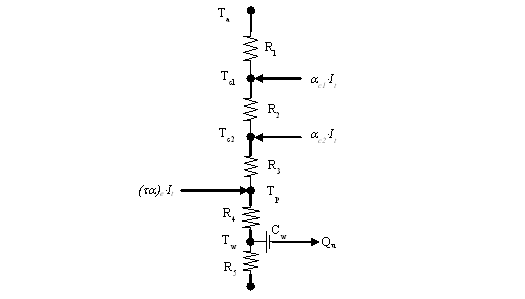
\includegraphics[width=0.9\textwidth, height=0.9\textheight, keepaspectratio=true]{media/image6522.png}
\caption{Thermal network diagram for ICS Solar Collector \protect \label{fig:thermal-network-diagram-for-ics-solar}}
\end{figure}

\textbf{\emph{Collector Cover Heat Balance}}

Ignoring the thermal mass of the collector cover, a steady state heat balance equations are formulated for each cover that allow us to determine cover temperatures.~ The cover surface heat balance representation is shown in Figure~\ref{fig:collector-cover-surface-heat-balance} below.

\begin{figure}[hbtp] % fig 297
\centering

\includegraphics[width=0.9\textwidth, height=0.9\textheight, keepaspectratio=true]{media/image6523.png}
\caption{Collector Cover Surface Heat Balance \protect \label{fig:collector-cover-surface-heat-balance}}
\end{figure}

The steady state cover heat balance equation is given by:

\begin{equation}
{q_{LWR,{\kern 1pt} 1}} + {q_{CONV,{\kern 1pt} 1}} + {q_{solar,{\kern 1pt} abs}} + {q_{LWR,{\kern 1pt} 2}} + {q_{CONV,{\kern 1pt} 2}} = 0
\end{equation}

Linearizing the longwave radiation exchange and representing the convection terms using the classical equation for Newton's law of cooling, the equations for the temperatures of covers 1 and 2 are given by:

\begin{equation}
{T_{c{\rm{1}}}} = \frac{{{\alpha_{c1}}{I_t} + {h_{r,{\kern 1pt} c1 - a}}{T_a} + {h_{c,{\kern 1pt} c1 - a}}{T_a} + {h_{r,{\kern 1pt} c2 - c1}}{T_{c2}} + {h_{c,{\kern 1pt} c2 - c1}}{T_{c2}}}}{{{h_{r,{\kern 1pt} c1 - a}} + {h_{c,{\kern 1pt} c1 - a}} + {h_{r,{\kern 1pt} c2 - c1}} + {h_{c,{\kern 1pt} c2 - c1}}}}
\end{equation}

\begin{equation}
{T_{c2}} = \frac{{{\alpha_{c2}}{I_t} + {h_{r,{\kern 1pt} c2 - c1}}{T_{c1}} + {h_{c,{\kern 1pt} c2 - c1}}{T_{c1}} + {h_{r,{\kern 1pt} p - c2}}{T_p} + {h_{c,{\kern 1pt} p - c2}}{T_p}}}{{{h_{r,{\kern 1pt} c2 - c1}} + {h_{c,{\kern 1pt} c2 - c1}} + {h_{r,{\kern 1pt} p - c2}} + {h_{c,{\kern 1pt} p - c2}}}}
\end{equation}

where:

\(\alpha_{c}\) is the weighted average solar absorptance of covers \emph{1} and \emph{2}

\(h_{r,c1-a}\) is the adjusted radiation heat transfer coefficient between cover \emph{1} and the ambient air (W/m\(^{2}\)-K)

\(h_{c,c1-a}\) is the convection heat transfer coefficient between cover \emph{1} and the ambient (W/m\(^{2}\)-K)

\(h_{r,c2-c1}\) is the radiation heat transfer coefficient between covers \emph{1} and \emph{2} (W/m\(^{2}\)-K)

\(h_{c,c2-c1}\) is the convection heat transfer coefficient between covers \emph{1} and \emph{2} (W/m\(^{2}\)-K)

\(h_{r,p-c2}\) is the radiation heat transfer coefficient between covers \emph{2} and the absorber plate (W/m\(^{2}\)-K)

\(h_{c,p-c2}\) is the convection heat transfer coefficient between covers \emph{2} and the absorber plate (W/m\(^{2}\)-K)

\(q_{LWR,1}\) is the longwave radiation exchange flux on side \emph{1} of the collector cover (W/m\(^{2}\))

\(q_{CONV,1}\) is the convection heat flux on side \emph{1} of the collector cover (W/m\(^{2}\))

\(q_{LWR,2}\) is the longwave radiation exchange flux on side \emph{2} of the collector cover (W/m\(^{2}\))

\(q_{CONV,2}\) is the convection heat flux on side \emph{2} of the collector cover (W/m\(^{2}\))

\(q_{solar,abs}\) is the net solar radiation absorbed by the collector cover (W/m\(^{2}\))

\(R\) is the thermal resistance for each section along the heat flow path (m\(^{2}\)K/W).

\subsubsection{Other Side Condition Model}\label{other-side-condition-model}

ICS Solar Collectors are commonly mounted on building heat transfer surfaces hence the collectors shade the underlying heat transfer surface and require a unique boundary condition that reflects the air cavity environment created between the bottom of the collector surface and the underlying surface. The other side condition model that allows us to estimate the other side temperature, \emph{T\(_{osc}\)}, can be determined based on steady state heat balance using the known collector water temperature at the previous time step.

\begin{figure}[hbtp] % fig 298
\centering

\includegraphics[width=0.9\textwidth, height=0.9\textheight, keepaspectratio=true]{media/image6527.png}
\caption{Illustration for Other Side Condition Model \protect \label{fig:illustration-for-other-side-condition-model}}
\end{figure}

Ignoring thermal mass of the collector bottom insulation, steady state surface heat balance can be formulated on the outer plane of the collector bottom surface facing the cavity as shown in Figure~\ref{fig:illustration-for-other-side-condition-model}.~ The heat balance equation on the outer plane of the collector bottom surface is given by:

\begin{equation}
{q_{cond}} + {q_{conv,{\kern 1pt} cav}} + {q_{rad,{\kern 1pt} cav}} = 0
\end{equation}

Substituting the equations for each term in the above equation yields:

\begin{equation}
U_L \left( T_w - T_{osc} \right) + h_{c,{\kern 1pt} cav} \left( T_{a,{\kern 1pt} cav} - T_{osc} \right) + h_{r,{\kern 1pt} cav} \left( T_{so} - T_{osc} \right) = 0
\end{equation}

Simplifying yields the bottom insulation other side condition temperature:

\begin{equation}
{T_{osc}} = \frac{{{U_L}{T_w} + {h_{c,{\kern 1pt} cav}}{T_{a,{\kern 1pt} cav}} + {h_{r,{\kern 1pt} cav}}{T_{so}}}}{{{U_L} + {h_{c,{\kern 1pt} cav}} + {h_{r,{\kern 1pt} cav}}}}
\end{equation}

The cavity air temperature is determined from cavity air heat balance as follows:

\begin{equation}
{T_{a,{\kern 1pt} cav}} = \frac{{{h_{c,{\kern 1pt} cav}}A{T_{osc}} + {{\dot m}_{vent}}Cp{T_a} + {h_{c,{\kern 1pt} cav}}A{T_{so}}}}{{{h_{c,{\kern 1pt} cav}}A + {{\dot m}_{vent}}Cp + {h_{c,{\kern 1pt} cav}}A}}
\end{equation}

where:

\(h_{r,cav}\) is the linearized radiation coefficient for underlying surface in the cavity (W/m\(^{2}\)-K)

\(h_{c,cav}\) is the convection coefficient for underlying surface in the cavity (W/m\(^{2}\)-K)

\(T_{so}\) is the outside face temperature of the underlying heat transfer surface (\(^{\circ}\)C)

\({\dot m_{vent}}\) is the air mass flow rate due to natural ventilation (kg/s)

\(q_{cond}\) is the conduction heat flux though the insulation and bottom (W/m\(^{2}\))

\(q_{conv,cav}\) is the convection heat flux between the collector bottom outside surface and the cavity air (W/m\(^{2}\))

\(q_{rad,cav}\) is the longwave radiation exchange flux between the collector bottom outside surface and the outside surface of the underlying surface (W/m\(^{2}\)).

The cavity air temperature is determined from the cavity air energy balance.~ The air heat balance requires the ventilated cavity air natural ventilation rates.~ The calculation of the ventilation rate is described else where in this document. The SurfaceProperty:ExteriorNaturalVentedCavity, object is required to describe the surface properties, the characteristics of the cavity and opening for natural ventilation.

\subsubsection{Heat Transfer Coefficients}\label{heat-transfer-coefficients}

The equations used to determine for the various heat transfer coefficients in the absorber and water heat balance equations are given below. The absorbed solar energy is transferred to the water by convection.~ Assuming natural convection dominated heat transfer for a hot surface facing down and a clod surface facing down the following correlation for Nusselt number by Fujii and Imura (1972).~ The Nusselt number for hot surface facing down ward is given by:

\begin{equation}
Nu = 0.56{\left( {Gr \cdot \Pr  \cdot cos{\kern 1pt} \theta } \right)^{1/5}}\quad {10^5} < Gr \cdot Pr < {10^{11}}
\end{equation}

The Nusselt number for hot surface upward and cold surface facing down is given by:

\begin{equation}
Nu = 0.13{\left( {Gr \cdot \Pr } \right)^{1/3}}\quad Gr \cdot Pr < 5.0 \times {10^8}
\end{equation}

\begin{equation}
Nu = 0.16{\left( {Gr \cdot \Pr } \right)^{1/3}}\quad Gr \cdot Pr > 5.0 \times {10^8}
\end{equation}

\begin{equation}
Gr = {{g{\beta_{\rm{v}}}\left( {{T_p} - {T_w}} \right)L_c^3} \mathord{\left/ {\vphantom {{g{\beta_{\rm{v}}}\left( {{T_p} - {T_w}} \right)L_c^3} {{\nu ^2}}}} \right. } {{\nu ^2}}}
\end{equation}

\begin{equation}
\Pr  = {\nu  \mathord{\left/ {\vphantom {\nu  \alpha }} \right. } \alpha }
\end{equation}

\begin{equation}
{T_r} = {T_p} - 0.25\left( {{T_p} - {T_w}} \right)
\end{equation}

\begin{equation}
{h_w} = {{Nu \cdot k} \mathord{\left/ {\vphantom {{Nu \cdot k} {{L_c}}}} \right. } {{L_c}}}
\end{equation}

where:

\(\theta\) is the angle of inclination of the collector to the vertical (radians)

\emph{g} is the gravitation force constant, 9.806 (m/s\(^{2}\))

\(T_{r}\) is the reference properties where the thermo-physical properties are calculated (\(^{\circ}\)C)

\(L_{c}\) is the characteristic length for the absorber plate (m)

\emph{k} is the thermal conductivity of water at reference temperature (W/m-K)

\({\nu}\) is the kinematic viscosity of water at reference temperature (m\(^{2}\)/s)

\(\alpha\) is the thermal diffusivity of water at reference temperature (m\(^{2}\)/s)

\(\beta_{v}\) is the volumetric expansion coefficient (1/K) evaluated at Tv, Tv = Tw+0.25(Tp-Tw)

\emph{Nu} is the Nusselt number calculated for water properties at the reference temperature

\emph{Gr} is the Grashof number calculated for water properties at the reference temperature

\emph{Pr} is the Prandtl number calculated for water properties at the reference temperature.

The various radiation and convection heat transfer coefficients are given by the following equations.~ The convection heat transfer coefficients between the covers and the absorber plate are estimated from the empirical correlation for the Nusselt number for air gap between two parallel plates developed by Hollands et al. (1976) is:

\begin{equation}
N{u_a} = 1 + 1.44\left\{ {1 - \frac{{1708{{\left( {\sin 1.8\beta } \right)}^{1.6}}}}{{Ra\cos \beta }}} \right\}{\left\{ {1 - \frac{{1708}}{{Ra\cos \beta }}} \right\}} + {\left\{ {{{\left( {\frac{{Ra\cos \beta }}{{5830}}} \right)}^{{\raise0.7ex\hbox{1} \!\mathord{\left/ {\vphantom {1 3}}\right.}\!\lower0.7ex\hbox{3}}}} - 1} \right\}}
\end{equation}

\begin{equation}
{h_c} = {{Nu \cdot k} \mathord{\left/ {\vphantom {{Nu \cdot k} L}} \right. } L}
\end{equation}

\begin{equation}
{h_{rp - c2}} = \frac{{\sigma \left( {{T_p} + {T_{c2}}} \right)\left( {T_p^2 + T_{c2}^2} \right)}}{{1/{\varepsilon_p} + 1/{\varepsilon_{c2}} - 1}}
\end{equation}

\begin{equation}
{h_{rc1 - c2}} = \frac{{\sigma \left( {{T_{c1}} + {T_{c2}}} \right)\left( {T_{c1}^2 + T_{c2}^2} \right)}}{{1/{\varepsilon_{c1}} + 1/{\varepsilon_{c2}} - 1}}
\end{equation}

The long wave radiation exchange coefficients between the outer collector cover and the sky and ground referencing the ambient air temperature for mathematical simplification are given.

\begin{equation}
{h_{rc1 - s}} = \frac{{{F_s}{\varepsilon_{c1}}\sigma \left( {{T_{c1}} + {T_s}} \right)\left( {T_{c1}^2 + T_s^2} \right)\left( {{T_{c1}} - {T_s}} \right)}}{{\left( {{T_{c1}} - {T_a}} \right)}}
\end{equation}

\begin{equation}
{h_{rc1 - g}} = \frac{{{F_g}{\varepsilon_{c1}}\sigma \left( {{T_{c1}} + {T_g}} \right)\left( {T_{c1}^2 + T_g^2} \right)\left( {{T_{c1}} - {T_g}} \right)}}{{\left( {{T_{c1}} - {T_a}} \right)}}
\end{equation}

\begin{equation}
{h_{cc1 - a}} = {h_{cc1 - s}} + {h_{cc1 - g}}
\end{equation}

The convection heat transfer coefficient from the outer cover to the surrounding air is given by:

\begin{equation}
{h_{cc1 - a}} = 2.8 + 3.0{V_w}
\end{equation}

When the bottom surface boundary condition is AmbientAir, the combined conductance from the outer cover to the surrounding is calculated from the equation below (Duffie and Beckman, 1991).

\begin{equation}
{h_{comb}} = 5.7 + 3.8{V_w}
\end{equation}

The overall loss coefficient through the bottom and side of the collector-storage is estimated as follows:

\begin{equation}
{U_b} = {U_{Lb}}\left( {{A_b}/A} \right)
\end{equation}

\begin{equation}
{U_s} = {\left[ {\frac{1}{{{U_{Ls}}\left( {{A_s}/A} \right)}} + \frac{1}{{{h_{comb}}}}} \right]^{ - 1}}
\end{equation}

where:

\({\varepsilon}_{c1}\) is the thermal emissivity of collector cover \emph{1}

\({\varepsilon}_{c2}\) is the thermal emissivity of collector cover \emph{2}

\(F_{s}\) is the view factor from the collector to the sky

\(F_{g}\) is the view factor from the collector to the ground

\(T_{c1}\) is the temperature of collector cover \emph{1}, (K)

\(T_{c2}\) is the temperature of collector cover \emph{2}, (K)

\(T_{s}\) is the sky temperature, (K)

\(T_{g}\) is the ground temperature, (K)

\emph{k} is the thermal conductivity of air (W/m K)

\emph{L} is the air gap between the covers (m)

\(\beta\) is the inclination of the plates or covers to the horizontal (radians)

\(V_{w}\) is the wind speed (m/s)

\(U_{Lb}\) is the user specified bottom heat loss conductance (W/m\(^{2}\)-K)

\(U_{Ls}\) is the user specified side heat loss conductance (W/m\(^{2}\)-K)

\(A_{b}\) is the collector bottom heat transfer area (m\(^{2}\))

\(A_{s}\) is the collector side area (m\(^{2}\))

\(h_{comb}\) is the combined conductance from the outer cover to the ambient air (W/m\(^{2}\)-K).

\textbf{\emph{Transmittance-Absorptance Product}}

The transmittance-absorptance product of solar collector is determined using ray tracing method for any incident angle (Duffie and Beckman, 1991).~ This requires optical properties of the cover and absorber materials and the the transmittance-absorptance product for any incident angle is given by:

\begin{equation}
{\left( {\tau \alpha } \right)_\theta } = \frac{{\tau \alpha }}{{1 - \left( {1 - \alpha } \right){\rho_d}}}
\end{equation}

The transmittance of the cover system for single and two cover are given by:

\begin{equation}
\tau  = \frac{1}{2}\left[ {{{\left( {\frac{{{\tau_1} \cdot {\tau_2}}}{{1 - {\rho_1}{\rho_2}}}} \right)}_ \bot } + {{\left( {\frac{{{\tau_1} \cdot {\tau_2}}}{{1 - {\rho_1}{\rho_2}}}} \right)}_\parallel }} \right]
\end{equation}

\begin{equation}
\rho  = \frac{1}{2}\left[ {{{\left( {{\rho_1} + \frac{{\tau  \cdot {\rho_2} \cdot {\tau_1}}}{{{\tau_2}}}} \right)}_ \bot } + {{\left( {{\rho_1} + \frac{{\tau  \cdot {\rho_2} \cdot {\tau_1}}}{{{\tau_2}}}} \right)}_\parallel }} \right]
\end{equation}

The effective transmittance, reflectance and absorptance of a single cover are given by:

\begin{equation}
\tau  = \frac{{{\tau_a}}}{2}\left\{ {\frac{{1 - {r_ \bot }}}{{1 + {r_ \bot }}}\left[ {\frac{{1 - r_ \bot ^2}}{{1 - {{\left( {{r_ \bot }{\tau_a}} \right)}^2}}}} \right] + \frac{{1 - {r_\parallel }}}{{1 + {r_\parallel }}}\left[ {\frac{{1 - r_\parallel ^2}}{{1 - {{\left( {{r_\parallel }{\tau_a}} \right)}^2}}}} \right]} \right\}
\end{equation}

\begin{equation}
\rho  = \frac{1}{2}\left\{ {\left[ {{r_ \bot } + \frac{{{{\left( {1 - {r_ \bot }} \right)}^2}\tau_a^2{r_ \bot }}}{{1 - {{\left( {{r_ \bot }{\tau_a}} \right)}^2}}}} \right] + \left[ {{r_\parallel } + \frac{{{{\left( {1 - {r_\parallel }} \right)}^2}\tau_a^2{r_\parallel }}}{{1 - {{\left( {{r_\parallel }{\tau_a}} \right)}^2}}}} \right]} \right\}
\end{equation}

\begin{equation}
\alpha  = \frac{{\left( {1 - {\tau_a}} \right)}}{2}\left\{ {\left( {\frac{{1 - {r_ \bot }}}{{1 - {r_ \bot }{\tau_a}}}} \right) + \left( {\frac{{1 - {r_\parallel }}}{{1 - {r_\parallel }{\tau_a}}}} \right)} \right\}
\end{equation}

The transmittance of the cover system with absorption only considered \emph{t}\(_{a}\), is defined as:

\begin{equation}
{\tau_a} = \exp \left( { - \frac{{KL}}{{\cos \,{\theta_2}}}} \right)
\end{equation}

\begin{equation}
{\theta_2} = {\sin ^{ - 1}}\left( {\sin {\theta_1} \cdot \frac{{{n_1}}}{{{n_2}}}} \right)
\end{equation}

The reflectance of un-polarized radiation on passing from medium 1 with reflective index \emph{n}\(_{1}\) to medium 2 with reflective index \emph{n}\(_{2}\) is given by:

\begin{equation}
{r_ \bot } = \frac{{{{\sin }^2}\left( {{\theta_2} - {\theta_1}} \right)}}{{{{\sin }^2}\left( {{\theta_2} + {\theta_1}} \right)}}
\end{equation}

\begin{equation}
{r_\parallel } = \frac{{{{\tan }^2}\left( {{\theta_2} - {\theta_1}} \right)}}{{{{\tan }^2}\left( {{\theta_2} + {\theta_1}} \right)}}
\end{equation}

The sky and ground reflected diffuse radiations average equivalent incident angles are approximated by Brandemuehl and Beckman correlation (Duffie and Beckman, 1991) as follows:

\begin{equation}
{\theta_{sd}} = 59.68 - 0.1388\beta  + 0.001497{\beta ^2}
\end{equation}

\begin{equation}
{\theta_{gd}} = 90 - 0.5788\beta  + 0.002693{\beta ^2}
\end{equation}

where:

\({\tau}\) is the transmittance of the cover system

\({\tau}_{1}\) is the transmittance of the cover 1

\({\tau}_{2}\) is the transmittance of the cover 2

\({\alpha}\) is the absorptance of the absorber plate

\({\rho}_{d}\) is the diffuse reflectance of the inner cover

\emph{L} is the thickness of a cover material (m)

\emph{K} is the extinction coefficient of a cover material (m\(^{-1}\))

\({\theta}_{1}\) is the angle of incidence (degrees)

\({\theta}_{2}\) is the angle of refraction (degrees)

\({r_ \bot }\) is the parallel component of reflected un-polarized radiation

\({r_\parallel }\) is the perpendicular component of reflected un-polarized radiation

\({\beta}\) is the slope of the collector (degrees)

\({\theta}_{sd}\) is the equivalent incident angle for sky diffuse solar radiation (degrees)

\({\theta}_{gd}\) is the equivalent incident angle for ground diffuse solar radiation (degrees).

The integral collector storage unit thermal performance parameters are calculated as follows:

\begin{equation}
{Q_{delivered}} = {\dot m_w}{C_w}\left( {{T_w} - {T_{wi}}} \right)
\end{equation}

\begin{equation}
{Q_{Stored}} = {m_w}{C_w}\frac{{d{T_w}}}{{dt}}
\end{equation}

\begin{equation}
{Q_{SkinLoss}} = A \cdot \left[ {{U_t}\left( {{T_p} - {T_w}} \right) + {U_b}\left( {{T_w} - {T_{OSC}}} \right) + {U_s}\left( {{T_w} - {T_a}} \right)} \right]
\end{equation}

\begin{equation}
{\eta_{thermal}} = \frac{{{m_w}{C_w}\frac{{d{T_w}}}{{dt}} + {{\dot m}_w}{C_w}\left( {{T_w} - {T_{wi}}} \right)}}{{A \cdot {I_t}}}
\end{equation}

\subsection{References:}\label{references-1-016}

Duffie, J.A., and W.A. Beckman. 1991. \emph{Solar Engineering of Thermal Processes,} 2d ed. New York: John Wiley \& Sons.

Kumar, R. and M.A.~Rosen. Thermal performance of integrated collector storage solar water heater with corrugated absorber surface. Applied Thermal Engineering:~ 30 (2010) 1764--1768.

Fujii, T., and H. Imura. Natural convection heat transfer from aplate with arbitrary inclination. International Journal of Heat and Mass Transfer: 15(4), (1972), 755-764.

\subsection{Photovoltaic Thermal Flat-Plate Solar Collectors}\label{photovoltaic-thermal-flat-plate-solar-collectors}

Photovoltaic-Thermal solar collectors (PVT) combine solar electric cells and thermal working fluid to collect both electricity and heat.~ Athough there are currently comparatively few commercial products, PVT research has been conducted for the past 30 years and many different types of collectors have been studied.~ Zondag (2008) and Charalambous et. al (2007) provide reviews of the PVT literature.~ Because PVT is much less commercially-mature, there are no standards or rating systems such as for thermal-only, hot-water collectors.~ EnergyPlus currently has one simple model based on user-defined efficiencies but a more detailed model based on first-principles and a detailed, layer-by-layer description is under development.

The PVT models reuse the PV models for electrical production. These are described elsewhere in this document in the section on Photovoltaic Arrays-Simple Model

\subsubsection{Simple PVT Thermal Model}\label{simple-pvt-thermal-model}

The input object SolarCollector:FlatPlate:PhotovoltaicThermal provides a simple PVT model that is provided for quick use during design or policy studies.~ The user simply provides values for a thermal efficiency and the incident solar heats the working fuild.~ The model also includes a cooling mode for air-based systems where a user-provided surface emmittance is used to model cooling of the working fluid to the night sky (water-based cooling will be made available once a chilled water storage tank is available).~ No other details of the PVT collector's construction are required as input data.

The simple model can heat either air or liquid.~ If it heats air, then the PVT is part of HVAC air system loop with air nodes connected to an air system.~ If it heats liquid, then the PVT is part of plant loop with nodes connected to a plant loop and the plant operating scheme determines flows.

Air-system-based PVT modeling include a modulating bypass damper arrangement.~ Control logic decides if the air should bypass the collector to better meet setpoint.~ The model requires a drybulb temperature setpoint be placed on the outlet node.~ The model assume the collector is intended and available for heating when the incident solar is greater than 0.3 W/m\(^{2}\) and otherwise it is intended for cooling.~ The inlet temperature is compare to the setpoint on the outlet node to determine if cooling or heating are beneficial.~ If they are, then the PVT thermal models are applied to condition the air stream.~ If they are not beneficial, then the PVT is completely bypassed and the inlet node is passed directly to the outlet node to model a completely bypassed damper arrangement.~ A report variable is available for bypass damper status.

Plant-based PVT do not include a bypass (although one could be used in the plant loop).~ The collector requests its design flow rate but it otherwise relies on the larger plant loop for control.

When the PVT themal collector is controlled to be ``on,'' in heating mode, and working fluid is flowing, the model calculates the outlet temperature based on the inlet temperature and the collected heat using the following equations.

\begin{equation}
{Q_{therm}} = {A_{surf}} \cdot {f_{activ}} \cdot {G_T} \cdot {\eta_{thermal}}
\end{equation}

where:

\({Q_{therm}}\) is the thermal energy collected (W)

\({A_{surf}}\) is the net area of the surface (m\(^{2}\))

\({f_{activ}}\) is the fraction of surface aire with active PV/T collector

\({\eta_{thermal}}\) is the thermal conversion efficiency.

\begin{equation}
{T_{out}} = {T_{in}} + \frac{{{Q_{therm}}}}{{\dot m{c_p}}}
\end{equation}

where:

\({T_{out}}\) is the temperature of the working fluid leaving the PV/T

\({T_{in}}\) is the temperature of the working fluid entering the PV/T

\(\dot m\) is the entire mass flow of the working fluid through the PV/T

\({c_p}\) is the specific heat of the working fluid.

For air-based systems, the value of \({T_{out}}\) is then compared to the temperature setpoint on the outlet node.~ If \({T_{out}}\) exceeds the desired outlet temperature, \({T_{set,out}}\), then a bypass fraction is calculated to model a modulating bypass damper using:

\begin{equation}
{f_{bypass}} = \frac{{\left( {{T_{set,out}} - {T_{out}}} \right)}}{{\left( {{T_{in}} - {T_{out}}} \right)}}
\end{equation}

When the PVT themal collector is controlled to be ``on,'' in cooling mode, and working fluid is flowing, the model calculates the outlet temperature based on the inlet temperature and the heat radiated and convected to the ambient using a heat balance on the outside face of the collector:

\begin{equation}
\dot m{c_p}\left( {{T_{in}} - {T_{out}}} \right) = {\dot Q_{LWR}} + {\dot Q_{conv}}
\end{equation}

where:

\({\dot Q_{LWR}}\) ~is the net rate of long wavelength (thermal) radiation exchange with the air, night sky, and ground.~ See the section ``External Longwave Radiation'' in the Outside Surface Heat Balance, for full discussion of how this modeled in EnergyPlus using linearized radiation coefficients.

\({\dot Q_{conv}}\) ~is the net rate of convective flux exchange with outdoor air. See the section ``Exterior/External Convection'' in the Outside Surface Heat Balance, for full discussion of how this modeled in EnergyPlus.~ The surface roughness is assumed to be ``very smooth.''

The simple model assumes that the effective collector temperature, \({T_{col}}\) , is the average of the working fluid inlet and outlet temperatures so that we can make the following substitution:

\begin{equation}
{T_{out}} = 2{T_{col}} - {T_{in}}
\end{equation}

Substituting and solving for \({T_{col}}\) ~we obtain the following model for collector temperatures during a (possible) cooling process :

\begin{equation}
{T_{col}} = \frac{{2\dot m{c_p}{T_{in}} + {A_{surf}}{f_{activ}}\left( {{h_{r,gnd}}{T_{gnd}} + {h_{r,sky}}{T_{sky}} + {h_{r,air}}{T_{air}} + {h_{c,ext}}{T_{air}}} \right)}}{{2\dot m{c_p} + {A_{surf}}{f_{activ}}\left( {{h_{r,gnd}} + {h_{r,sky}} + {h_{r,air}} + {h_{c,ext}}} \right)}}
\end{equation}

Then the outlet temperature can be calculated and heat losses determined.~ However, the model allows only sensible cooling of the air stream and limits the outlet temperature to not go below the dewpoint temperature of the inlet.

PVT collectors have a design volume flow rate for the working fluid that is autosizable.~ For air-based systems used as pre-conditioners, the volume flow rate is sized to meet the maximum outdoor air flow rate.~ For water-based systems on the supply side of a plant loop, each of the PVT collectors are sized to the overall loop flow rate.~ For water-based systems on the demand side of a plant loop, the collectors are sized using a rule-of-thumb for typical flow rates per unit of collector area.~ This rule-of-thumb is based on a constant factor of 1.905x10\(^{-5}\) m\(^{3}\)/s-m\(^{2}\) that was developed by analyzing SRCC data set for conventional solar collectors (see data set SolarCollectors.idf) and averaging the ratio for all 171 different collectors.

\subsubsection{References}\label{references-2-008}

Charalambous, P.G., Maidment, G.G., Kalagirou, S.A., and Yiakoumetti, K., Photovoltaic thermal (PV/T) collectors: A review. Applied Thermal Engineering 27 (2007) 275-286.

Zondag, H.A. 2008. Flat-plate PV-Thermal collectors and systems: A review.~ Renewable and Sustainable Energy Reviews 12 (2008) 891-959.

\subsection{Unglazed Transpired Solar Collectors}\label{unglazed-transpired-solar-collectors}

The input object SolarCollector:UnglazedTranspired provides a model for transpired collectors that are perhaps one of the most efficient ways to collect solar energy with demonstrated instantaneous efficiencies of over 90\% and average efficiencies of over 70\%.~ They are used for preheating outdoor air needed for ventilation and processes such as crop drying.

In EnergyPlus, an unglazed transpired solar collector (UTSC) is modeled as a special component attached to the outside face of a heat transfer surface that is also connected to the outdoor air path.~ A UTSC affects both the thermal envelope and the HVAC air system.~ From the air system's point of view, a UTSC is heat exchanger and the modeling needs to determine how much the device raises the temperature of the outdoor air.~ From the thermal envelope's point of view, the presence of the collector on the outside of the surface modifies the conditions experienced by the underlying heat transfer surfaces.~ EnergyPlus models building performance throughout the year and the UTSC will often be ``off'' in terms of forced airflow, but the collector is still present.~ When the UTSC is ``on'' there is suction airflow that is assumed to be uniform across the face.~ When the UTSC is ``off'' the collector acts as a radiation and convection baffle situated between the exterior environment and the outside face of the underlying heat transfer surface.~ We distinguish these two modes of operation as \emph{active} or \emph{passive} and model the UTSC component differently depending on which of these modes it is in.

\subsubsection{Heat Exchanger Effectiveness}\label{heat-exchanger-effectiveness}

The perforated absorber plate is treated as a heat exchanger and modeled using a traditional effectiveness formulation.~ The heat exchanger effectiveness, \({\varepsilon_{HX}}\) , is determined from correlations derived from small-scale experiments.~ Two correlations available in the literature are implemented in EnergyPlus.~ The first is based on research by Kutscher at the National Renewable Energy Laboratory. The second is based on the research by Van Decker, Hollands, and Brunger at the University of Waterloo.~ Because both correlations are considered valid, the choice of which correlation to use is left to the user.

\subsubsection{Kutscher Correlation}\label{kutscher-correlation}

Kutscher's (1994) correlation encompasses surface convection between the collector and the incoming outdoor air stream that occurs on the front face, in the holes, and along the back face of the collector. The correlation uses a Reynolds number based on the hole diameter as a length scale and the mean velocity of air as it passes through the holes as the velocity scale:

\begin{equation}
{Re_D} = \frac{{{V_h}D}}{\nu }
\end{equation}

where:

\({V_h}\) is the velocity through the holes (m/s)

\(D\) is the hole diameter (m)

\(\nu\) is the kinematic viscosity of air (m\(^{2}\)/s).

The correlation is a function of Reynolds number, hole geometry, the free stream air velocity, and velocity through the holes:

\begin{equation}
N{u_D} = 2.75\left[ {{{\left( {\frac{P}{D}} \right)}^{ - 1.2}}{\mathop{\rm Re}\nolimits}_D^{0.43} + 0.011\sigma {{{\mathop{\rm Re}\nolimits} }_D}{{\left( {\frac{{{U_\infty }}}{{{V_h}}}} \right)}^{0.48}}} \right]
\end{equation}

where:

\(P\) is the pitch, or distance between holes (m)

\(D\) is the diameter of the holes (m)

\(\sigma\) is the porosity, or area fraction of the holes

\({V_h}\) is the mean velocity of air passing through the holes (m/s)

\({U_\infty }\) is the free stream velocity or the local wind speed (m/s).

The Nusselt number is formulated as:

\begin{equation}
N{u_D} = \frac{{U~D}}{k}
\end{equation}

where:

\(U\) is the overall heat transfer coefficient based on log mean temperature difference (W/m\(^{2}\)-K)

\(k\) is the thermal conductivity of air (W/m-K).

The heat exchanger effectiveness is:

\begin{equation}
{\varepsilon_{HX}} = 1 - {e^{\left[ { - \frac{{U~A}}{{\dot m~{c_p}}}} \right]}}
\end{equation}

Kutscher's relation was formulated for triangular hole layout, but based on Van Decker et al. (2001) we allow using the correlation for square hole layout and scale \(P\) by a factor of 1.6.

\subsubsection{Van Decker, Hollands, and Brunger Correlation}\label{van-decker-hollands-and-brunger-correlation}

Van Decker et. al. extended Kutscher's measurements to include a wider range of collector parameters including plate thickness, pitch, suction velocities, and square hole patterns.~ Their model formulation differs from Kutscher's in that the model was built up from separate effectiveness models for the front, back, and holes of the collector.~ Their published correlation is:

\begin{equation}
\begin{split}
{\varepsilon_{HX}} =& \left[ {1 - \left( {1 + {{{\mathop{\rm Re}\nolimits} }_s}Max{{\left( {1.733{\mathop{\rm Re}\nolimits}_w^{ - {\raise0.7ex\hbox{1} \!\mathord{\left/ {\vphantom {1 2}}\right.}\!\lower0.7ex\hbox{2}}},0.02136} \right)}^{ - 1}}} \right)} \right] \times \left[ {1 - {{\left( {1 + 0.2273{\mathop{\rm Re}\nolimits}_b^{{\raise0.7ex\hbox{1} \!\mathord{\left/ {\vphantom {1 2}}\right.}\!\lower0.7ex\hbox{2}}}} \right)}^{ - 1}}} \right] \\
&\times {e^{\left( { - 0.01895\frac{P}{D} - \frac{{20.62}}{{{{{\mathop{\rm Re}\nolimits} }_D}}}\frac{t}{D}} \right)}}
\end{split}
\end{equation}

where:

\begin{equation}
{Re_s} = \frac{{{V_s}P}}{v}
\end{equation}

\begin{equation}
{Re_w} = \frac{{{U_\infty }P}}{v}
\end{equation}

\begin{equation}
{Re_b} = \frac{{{V_h}P}}{v}
\end{equation}

\({V_s}\) is the average suction velocity across the front face of the collector (m/s)

\(t\) is the collector plate thickness (m).

\subsubsection{Heat Exchanger Leaving Temperature}\label{heat-exchanger-leaving-temperature}

Using either of the correlations above allows determining the heat exchanger effectiveness from known values.~ By definition the heat exchanger effectiveness is also:

\begin{equation}
{\varepsilon_{HX}} = \frac{{{T_{a,HX}} - {T_{amb}}}}{{{T_{s,coll}} - {T_{amb}}}}
\label{eq:SolarCollectorHXEffect716}
\end{equation}

where:

\({T_{{\rm{a,HX}}}}\) is the temperature of the air leaving the collector and entering the plenum (\(^{\circ}\)C)

\({T_{s,coll}}\) is the temperature of the collector's absorber plate (\(^{\circ}\)C)

\({T_{amb}}\) is the temperature of the ambient outdoor air (\(^{\circ}\)C).

By rewriting Equation~\ref{eq:SolarCollectorHXEffect716} to solve for \({T_{{\rm{a,HX}}}}\), we see that the temperature of the heated outdoor air entering the plenum can be determined once the collector surface temperature is known:

\begin{equation}
{T_{a,HX}} = {\varepsilon_{HX}}{T_{s,coll}} + \left( {1 - {\varepsilon_{HX}}} \right){T_{amb}}
\end{equation}

\subsubsection{Collector Heat Balance}\label{collector-heat-balance}

The collector is assumed to be sufficiently thin and high-conductivity so that it can be modeled using a single temperature (for both sides and along its area).~ This temperature \({T_{s,coll}}\) is determined by formulating a heat balance on a control volume that just encapsulates the collector surface.~ The heat balances are formulated separately for active and passive modes and are diagrammed in the following figure.

Observe that for the passive case, we do not use the heat exchanger relations to directly model the interaction of ventilating air with the collector.~ This is because these relations are considered to not apply when the UTSC is in passive mode.~ They were developed for uni-directional flow (rather than the balanced-in-and-out flow expected from natural forces) and for specific ranges of suction face velocity.~ Therefore, this heat transfer mechanism is handled using classical surface convection models (as if the collector was not perforated).~ (Air exchanges are modeled as ventilation in the plenum air heat balance but do not interact with the hole edges in the collector surface.)

\begin{figure}[hbtp] % fig 299
\centering
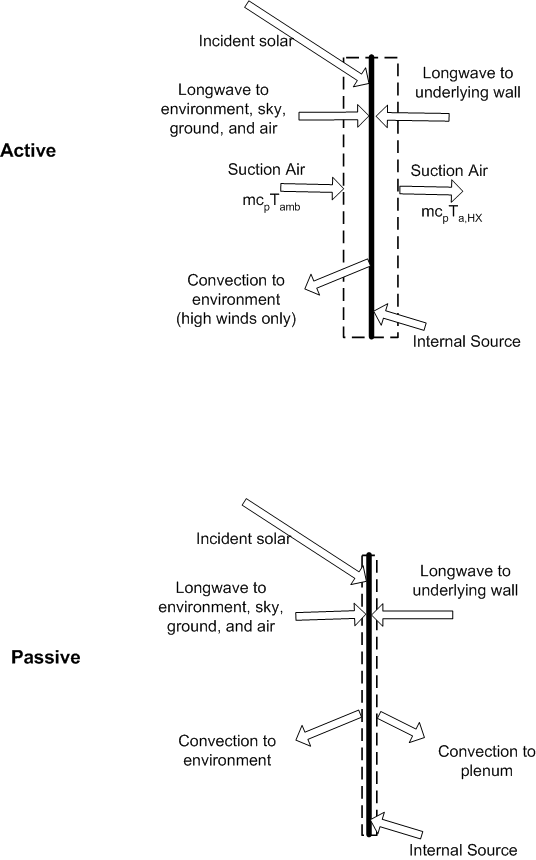
\includegraphics[width=0.9\textwidth, height=0.9\textheight, keepaspectratio=true]{media/image6620.png}
\caption{Transpired Collector Heat Balance \protect \label{fig:transpired-collector-heat-balance}}
\end{figure}

When the UTSC is active, the heat balance on the collector surface control volume is:

\begin{equation}
{q''_{\alpha sol}} + {q''_{LWR,Env}} + {q''_{conv,wind}} - {q''_{HX}} + {q''_{LWR,plen}} + {q''_{source}} = 0
\label{eq:SolarCollectorHeatBalance718}
\end{equation}

where:

\(q''_{\alpha sol}\) is absorbed direct and diffuse solar (short wavelength) radiation heat flux.

\({q''_{LWR,Env}}\) is net long wavelength (thermal) radiation flux exchange with the air and surroundings.

\({q''_{conv,wind}}\) is surface convection flux exchange with outdoor air under high wind and rain conditions.~ Note that this term is usually assumed to be zero in UTSC model development but we add the term to allow for deteriorated performance of the UTSC under poor conditions.

\(q''_{HX}\) is heat exchanger flux from collector to incoming outdoor air.

\(q''_{LWR,plen}\) is net long wavelength (thermal) radiation flux exchange with the outside face of the underlying surface(s).

\({q''_{source}}\) is a source/sink term that accounts for energy exported out of the control volume when the collecter's absorber plate is a hybrid device such as a photovoltaic panel.

While the heat balance on the passive collector surface control volume is:

\begin{equation}
{q''_{\alpha sol}} + {q''_{LWR,Env}} + {q''_{conv,Env}} + {q''_{LWR,plen}} + {q''_{conv,plen}} + {q''_{source}} = 0
\end{equation}

where:

\(q''_{conv,Env}\) is the surface convection flux exchange with outdoor air

\(q''_{conv,plen}\) is the surface convection flux exchange with plenum air.

All terms are positive for net flux to the collector except the heat exchanger term, which is taken to be positive in the direction from collector to incoming air stream.~ Each of these heat balance components is introduced briefly below.

\subsubsection{External SW Radiation}\label{external-sw-radiation-000}

\(q''_{\alpha sol}\) is calculated using procedures presented elsewhere in this manual and includes both direct and diffuse incident solar radiation absorbed by the surface face.~ This is influenced by location, surface facing angle and tilt, shading surfaces, surface face material properties, weather conditions, etc.

\subsubsection{External LW Radiation}\label{external-lw-radiation-000}

\({q''_{LWR,Env}}\) is a standard radiation exchange formulation between the surface, the sky, the ground, and the atmosphere.~ The radiation heat flux is calculated from the surface absorptivity, surface temperature, sky, air, and ground temperatures, and sky and ground view factors.~ Radiation is modeled using linearized coefficients.

\subsubsection{External Convection}\label{external-convection-000}

\(q''_{conv,Env}\) is modeled using the classical formulation:

\begin{equation}
{q''_{conv}} = {h_{co}}(T_{air} - T_{o})
\end{equation}

where h\(_{co}\) is the convection coefficient.~ This coefficient will differ depending on whether or not the UTSC is active or passive.~ When the UTSC is passive, h\(_{co}\) is treated in the same way as an outside face with ExteriorEnvironment conditions.~ When the UTSC is active, the special suction airflow situation of a transpired collector during operation means that h\(_{co}\) is often zero because the suction situation can eliminate mass transport away from the collector.~ However when the winds are high, the strong turbulence and highly varying pressures can cause the suction flow situation to breakdown.~ Therefore, we include the \({q''_{conv,wind}}\) term in the heat balance and use a special coefficient \({h_{c,wind}}\) to model this lost heat transfer.~ In addition, when it is raining outside, we assume the collector gets wet and model the enhanced surface heat transfer using a large value for \({h_{c,wind}}\).

\subsubsection{Heat Exchanger}\label{heat-exchanger}

\(q''_{HX}\) is modeled using the classical formulation:

\begin{equation}
{q''_{HX}} = \frac{{\dot m{c_p}({T_{a,HX}} - {T_{amb}})}}{A}
\end{equation}

where \({T_{{\rm{a,HX}}}}\) is determined using correlations described above.~ When the UTSC is active, the air mass flow is determined from the operation of the outdoor air mixer component.~ When the UTSC is off, this term is zero.

\subsubsection{Plenum LW Radation}\label{plenum-lw-radation}

\({q''_{LWR,plen}}\) is a standard radiation exchange formulation between the collector surface and the underlying heat transfer surface located across the plenum.~ Radiation is modeled using linearized coefficients.

\subsubsection{Plenum Convection}\label{plenum-convection}

\(q''_{conv,plen}\) is modeled using the classical formulation:

\begin{equation}
{q''_{conv}} = {h_{cp}}(T_{air} - T_{o})
\end{equation}

where h\(_{cp}\) is the convection coefficient.~ This coefficient is taken as zero when the UTSC is operating because of the suction airflow situation.~ When the UTSC is off, the value for h\(_{cp}\) is obtained from correlations used for window gaps from ISO (2003) standard 15099.

Substituting these models into Equation~\ref{eq:SolarCollectorHeatBalance718} and solving for \({T_{s,coll}}\) yields the following equation when the UTSC is active (``on''):

{\scriptsize
\begin{equation}
{T_{s,coll}} = \frac{{\left( {{I_s}\alpha  + {h_{r,atm}}{T_{amb}} + {h_{r,sky}}{T_{sky}} + {h_{r,gnd}}{T_{amb}} + {h_{r,plen}}{T_{so}} + {h_{c,wind}}{T_{amb}} + \frac{{\dot m{c_p}}}{A}{T_{amb}} - \frac{{\dot m{c_p}}}{A}\left( {1 - {\varepsilon_{HX}}} \right){T_{amb}} + {{q''}_{source}}} \right)}}{{\left( {{h_{r,atm}} + {h_{r,sky}} + {h_{r,gnd}} + {h_{r,plen}} + {h_{c,wind}} + \frac{{\dot m{c_p}}}{A}{\varepsilon_{HX}}} \right)}}
\end{equation}}

and substituting into Equation~\ref{eq:SolarCollectorHeatBalance718} yields the following equation when the UTSC is passive (``off''):

\begin{equation}
{T_{s,coll}} = \frac{{\left( {{I_s}\alpha  + {h_{co}}{T_{amb}} + {h_{r,atm}}{T_{amb}} + {h_{r,sky}}{T_{sky}} + {h_{r,gnd}}{T_{amb}} + {h_{r,plen}}{T_{so}} + {h_{c,plen}}{T_{a,plen}} + {{q''}_{source}}} \right)}}{{\left( {{h_{co}} + {h_{r,air}} + {h_{r,sky}} + {h_{r,gnd}} + {h_{r,plen}} + {h_{c,plen}}} \right)}}
\end{equation}

where:

\({I_s}\) is the incident solar radiation of all types (W/m\(^{2}\))

\(\alpha\) is the solar absorptivity of the collector

\({h_{r,atm}}\) is the linearized radiation coefficient for the surrounding atmosphere (W/m\(^{2}\)-K)

\({T_{amb}}\) is the outdoor drybulb from the weather data, also assumed for ground surface (\(^{\circ}\)C)

\({h_{r,sky}}\) is the linearized radiation coefficient for the sky (W/m\(^{2}\)-K)

\({T_{sky}}\) is the effective sky temperature (\(^{\circ}\)C)

\({h_{r,gnd}}\) is the linearized radiation coefficient for the ground (W/m\(^{2}\)-K)

\({h_{r,plen}}\) is the linearized radiation coefficient for the underlying surface (W/m\(^{2}\)-K)

\({h_{c,wind}}\) is the convection coefficient for the outdoor environment when the UTSC is active and winds are high or it is raining (W/m\(^{2}\)-K)

\({T_{so}}\) is the temperature of the outside face of the underlying heat transfer surface (\(^{\circ}\)C)

\(\dot m\) is the air mass flow rate when in active mode (kg/s)

\({c_p}\) is the specific heat of air at constant pressure (J/kg-K)

\(A\) is the area of the collector (m\(^{2}\))

\({h_{co}}\) is the convection coefficient for the outdoor environment (W/m\(^{2}\)-K)

\({h_{c,plen}}\) is the convection coefficient for the surfaces facing the plenum (W/m\(^{2}\)-K)

\({T_{a,plen}}\) is the air drybulb for air in the plenum and entering the outdoor air system (\(^{\circ}\)C).

\subsubsection{Plenum Heat Balance}\label{plenum-heat-balance}

The \emph{plenum} is the volume of air located between the collector and the underlying heat transfer surface.~ The plenum air is modeled as well-mixed.~ The uniform temperature of the plenum air, \({T_{a,plen}}\), is determined by formulating a heat balance on a control volume of air as diagrammed below.

Note that we have formulated the control volumes with slight differences for the active and passive cases.~ For the active case, the suction air situation and heat exchanger effectiveness formulations dictate that the collector surface control volume encompass part of the air adjacent to both the front and back surfaces of the collector.~ However for the passive case, the collector surface control volume has no air in it and the plenum air control volume extends all the way to the surface of the collector.

\begin{figure}[hbtp] % fig 300
\centering

\includegraphics[width=0.9\textwidth, height=0.9\textheight, keepaspectratio=true]{media/image6664.png}
\caption{Transpired Collector Plenum Air Heat Balance \protect \label{fig:transpired-collector-plenum-air-heat-balance}}
\end{figure}

When the UTSC is active, the heat balance on the plenum air control volume is:

\begin{equation}
  \dot{Q}_{air} + \dot{Q}_{co} = 0
\label{eq:SolarCollectorHeatBalancePlenumAir722}
\end{equation}

where:

\({\dot Q_{air}}\) is the net rate of energy added by suction air convecting through the control volume

\(\dot{Q}_{co}\) is the net rate of energy added by surface convection heat transfer with the underlying surface.

When the UTSC is passive, the heat balance on the plenum air control volume is:

\begin{equation}
{\dot Q_{vent}} + {\dot Q_{co}} + {\dot Q_{c,coll}} = 0
\end{equation}

where:

\({\dot Q_{vent}}\) is the net rate of energy added from infiltration -- where outdoor ambient air exchanges with the plenum air

\({\dot Q_{c,coll}}\) is the net rate of energy added by surface convection heat transfer with the collector.

Substituting into Equation~\ref{eq:SolarCollectorHeatBalancePlenumAir722} and solving for \({T_{a,plen}}\) yields the following equation for when the UTSC is active:

\begin{equation}
{T_{a,plen}} = \frac{{\left( {\dot m{c_p}{T_{a,HX}} + {h_{c,plen}}A\,{T_{so}}} \right)}}{{\left( {\dot m{c_p} + {h_{c,plen}}A} \right)}}
\end{equation}

And substituting into Equation~\ref{eq:SolarCollectorHeatBalancePlenumAir722} yields the following equation when the UTSC is passive:

\begin{equation}
{T_{a,plen}} = \frac{{\left( {{h_{c,plen}}A\,{T_{so}} + {{\dot m}_{vent}}{c_p}{T_{amb}} + {h_{c,plen}}A\,{T_{s,coll}}} \right)}}{{\left( {{h_{c,plen}}A + {{\dot m}_{vent}}{c_p} + {h_{c,plen}}A} \right)}}
\end{equation}

where \({\dot m_{vent}}\) is the air mass flow from natural forces (kg/s).

The literature on UTSC does not appear to address the passive mode of operation and no models for \({\dot m_{vent}}\) have been identified.~ Nevertheless, natural buoyancy and wind forces are expected to drive air exchange between the plenum and ambient and some method of modeling \({\dot m_{vent}}\) is needed.~ Reasoning that the configuration is similar to single-side natural ventilation, we elect to use correlations for natural ventilation presented in Chapter 26 of the ASHRAE Handbook of Fundamentals (2001).

\begin{equation}
{\dot m_{vent}} = \rho {{\rm{\rlap{--} \dot V}}_{{\rm{tot}}}}
\end{equation}

where:

\(\rho\) is the density of air (kg/m\(^{3}\))

\({{\rm{\rlap{--} \dot V}}_{{\rm{tot}}}} = {{\rm{\rlap{--} \dot V}}_{{\rm{wind}}}} + \,{{\rm{\rlap{--} \dot V}}_{{\rm{thermal}}}}\) is the total volumetric flow rate of air ventilating in and out of the plenum (m\(^{3}\)/s)

\begin{equation}
{{\rm{\rlap{--} \dot V}}_{{\rm{wind}}}} = {C_v}{A_{in}}{U_\infty }
\end{equation}

\begin{equation}
{{\rm{\rlap{--} \dot V}}_{{\rm{thermal}}}} = {C_D}{A_{in}}\sqrt {2g\Delta {H_{NPL}}\left( {{T_{a,plen}} - {T_{amb}}} \right)/{T_{a,plen}}} ~ (if~{T_{a,plen}} > {T_{amb}} )
\end{equation}

\begin{equation}
{{\rm{\rlap{--} \dot V}}_{{\rm{thermal}}}} = {C_D}{A_{in}}\sqrt {2g\Delta {H_{NPL}}\left( {{T_{amb}} - {T_{a,plen}}} \right)/{T_{amb}}} ~ (if~{T_{amb}} > {T_{a,plen}} ~ and~UTSC~vertical)
\end{equation}

where:

\({C_v}\) is the effectiveness of the openings that depends on opening geometry and the orientation with respect to the wind.~ ASHRAE HoF (2001) indicates values ranging from 0.25 to 0.6.~ In the UTSC model, this value is available for user input and defaulted to 0.25.

\({C_D}\) is the discharge coefficient for the opening and depends on opening geometry.~ In the UTSC model, this value is available for user input and defaulted to 0.65.

Mass continuity arguments lead to modeling the area of the openings as one half of the total area of the holes, so we have:

\begin{equation}
{A_{in}} = \frac{{A\,\sigma }}{2}
\end{equation}

\(g\) is the gravitational constant taken as 9.81 (m/s\(^{2}\)).

\(\Delta {H_{NPL}}\) is the height from midpoint of lower opening to the Neutral Pressure Level.~ This is taken as one-fourth the overall height of the UTSC if it is mounted vertically.~ For tilted collectors, the nominal height is modified by the sine of the tilt.~ If the UTSC is mounted horizontally (e.g.~on the roof) then the \(\Delta {H_{NPL}}\) is taken as the gap thickness of the plenum.

If the UTSC is horizontal and \({T_{amb}} > {T_{a,plen}}\), then \({{\rm{\rlap{--} \dot V}}_{{\rm{thermal}}}}{\rm{ = 0}}\) because this is a stable situation.

\subsubsection{Underlying Heat Transfer Surface}\label{underlying-heat-transfer-surface-000}

The UTSC is applied to the outside of a heat transfer surface.~ This surface is modeled using the usual EnergyPlus methods for handling heat capacity and transients -- typically the CTF method.~ These native EnergyPlus Heat Balance routines are used to calculate \({T_{so}}\) .~ The UTSC model is coupled to the underlying surface using the OtherSideConditionsModel mechanism.~ The UTSC model provides values for \({h_{r,plen}}\), \({T_{s,coll}}\), \({h_{c,plen}}\), and \({T_{a,plen}}\) for use with the Heat Balance Model calculations for the outside face of the underlying surface (described elsewhere in this manual).

\subsubsection{Solar and Shading Calculations}\label{solar-and-shading-calculations-2}

The transpired collector object uses a standard EnergyPlus surface in order to take advantage of the detailed solar and shading calculations.~ Solar radiation incident on the surface includes beam and diffuse radiation, as well as radiation reflected from the ground and adjacent surfaces.~ Shading of the collector by other surfaces, such as nearby buildings or trees, is also taken into account.

\subsubsection{Local Wind Speed Calculations}\label{local-wind-speed-calculations-000}

The outdoor wind speed affects terms used in modeling UTSC components.~ The wind speed in the weather file is assumed to be measured at a meteorological station located in an open field at a height of 10 m.~ To adjust for different terrain at the building site and differences in the height of building surfaces, the local wind speed is calculated for each surface.

The wind speed is modified from the measured meteorological wind speed by the equation (ASHRAE 2001):

\begin{equation}
{U_\infty } = {V_{met}}{\left( {\frac{{{\delta_{met}}}}{{{z_{met}}}}} \right)^{{a_{met}}}}{\left( {\frac{z}{\delta }} \right)^a}
\end{equation}

where:

\(z\) is the height of the centroid of the UTSC

\(z_{met}\) is the height of the standard metereological wind speed measurement

\(a\) and \({\delta}\) are terrain-dependent coefficients.~ \({\delta}\) is the boundary layer thickness for the given terrain type.~ The values of a and \({\delta}\) are shown in the Table~\ref{table:terrain-dependent-coefficients-ashrae-2001.-001}.

% table 77
\begin{longtable}[c]{@{}llll@{}}
\caption{Terrain-Dependent Coefficients (ASHRAE 2001). \label{table:terrain-dependent-coefficients-ashrae-2001.-001}} \tabularnewline
\toprule 
Terrain & Description & Exponent, a & Layer Thickness, $\delta$ (m) \tabularnewline
\midrule
\endfirsthead

\caption[]{Terrain-Dependent Coefficients (ASHRAE 2001).} \tabularnewline
\toprule 
Terrain & Description & Exponent, a & Layer Thickness, $\delta$ (m) \tabularnewline
\midrule
\endhead

1 & Flat, open country & 0.14 & 270 \tabularnewline
2 & Rough, wooded country & 0.22 & 370 \tabularnewline
3 & Towns and cities & 0.33 & 460 \tabularnewline
4 & Ocean & 0.10 & 210 \tabularnewline
5 & Urban, industrial, forest & 0.22 & 370 \tabularnewline
\bottomrule
\end{longtable}

The UTSC can be defined such that it has multiple underlying heat transfer surfaces.~ The centroid heights for each surface are area-weighted to determine the average height for use in the local wind calculation.

\subsubsection{Convection Coefficients}\label{convection-coefficients-000}

UTSC modeling requires calculating up to three different coefficients for surface convection heat transfer.~ These coefficients are defined in the classic way by:

\begin{equation}
{h_c} = \frac{{{T_{air}} - {T_{surf}}}}{{{{q''}_{conv}}}}
\end{equation}

First, \({h_{co}}\) is the convection coefficient for the collector surface facing the outdoors when the UTSC is passive.~ It is modeled in exactly the same way as elsewhere in EnergyPlus and will depend on the user setting for Outside Convection Algorithm -- Outside Surface Heat Balance entry elsewhere in this document.

Second, \({h_{c,plen}}\) is the convection coefficient for surfaces facing the plenum.~ This coefficient is applied to just the underlying surface's convection when the UTSC is active and to both the collector and the underlying surface when the UTSC is passive.~ When the UTSC is active, we use the convection correlation for forced air developed by McAdams (1954) as published by ASHRAE HoF (2001):

\begin{equation}
{h_{c,plen}} = 5.62 + 3.9{V_p}
\end{equation}

where \({V_p}\) is the mean velocity in the plenum determined from:

\begin{equation}
{V_p} = \frac{{\dot m}}{{2\rho {A_p}}}
\end{equation}

and where \({A_p}\) is the effective cross section area of the plenum perpendicular to the primary flow direction.~ When the UTSC is passive, we model the convection in the same way used in EnergyPlus to model air gaps in windows.~ These correlations vary by Rayleigh number and surface tilt and are based on the work of various research including Hollands et. al., Elsherbiny et. al., Wright, and Arnold.~ The formulations are documented in ISO (2003) standard 15099.~ For the UTSC implementation, the routines were adapted from Subroutine NusseltNumber in WindowManager.f90 (by F. Winkelmann), which itself was derived from Window5 subroutine ``nusselt''.

Third, \({h_{c,wind}}\) is the convection coefficient used to degrade the UTSC performance under environmental conditions with high wind or rain.~ If the weather file indicates it is raining, then we set \({h_{c,wind}}\) = 1000.0 which has the effect of making the collector the same temperature as ambient air.~ The heat exchanger effectiveness correlations described above account for a moderate amount of wind, but the correlations appear confined to the range 0 to 5.0 m/s.~ Therefore we set \({h_{c,wind}}\) equal to zero if \({U_\infty }\) is \textless{} = 5.0 m/s.~ If \({U_\infty }\) is \textgreater{} 5.0 m/s, then we use the McAdams correlation but with a reduced velocity magnitude:

\begin{equation}
{h_{c,wind}} = 5.62 + 3.9({U_\infty } - 5.0)
\end{equation}

\subsubsection{Radiation Coefficients}\label{radiation-coefficients-000}

UTSC modeling requires calculating up to four different linearized coefficients for radiation heat transfer.~ Whereas radiation calculations usually use temperature raised to the fourth power, this greatly complicates solving heat balance equations for a single temperature.~ Linearized radiation coefficients have the same units and are used in the same manner as surface convection coefficients and introduce very little error for the temperature levels involved.

The radiation coefficient, \({h_{r,plen}}\), is used to model thermal radiation between the collector surface and the outside face of the underlying heat transfer surface.~ We assume a view factor of unity.~ It is calculated using:

\begin{equation}
{h_{r,plen}} = {\sigma_{SB}}{e_{coll}}{e_{so}}\frac{{\left( {T_{s,coll}^4 - T_{so}^4} \right)}}{{\left( {{T_{s,coll}} - {T_{so}}} \right)}}
\end{equation}

where all temperatures are converted to Kelvin and:

\({\sigma_{SB}}\) is the Stefan-Boltzmann constant

\({e_{coll}}\) is the longwave thermal emmittance of the collector

\({e_{so}}\) is the longwave thermal emmittance of the underlying heat transfer surface.

The three other coefficients, \({h_{r,atm}}\), \({h_{r,sky}}\), and \({h_{r,gnd}}\) are used elsewhere in EnergyPlus for the outside face surface heat balance and are calculated in the same manner as equation for UTSC collectors.~ {[}This is accomplished by calling subroutine InitExteriorConvectionCoeffs in the file HeatBalanceConvectionCoeffs.f90.{]}

\subsubsection{Bypass Control}\label{bypass-control}

The UTSC is assumed to be arranged so that a bypass damper controls whether or not air is drawn directly from the outdoors or through the UTSC.~ The control decision is based on whether or not it will be beneficial to heat the outdoor air.~ There are multiple levels of control including an availability schedule, whether or not the outdoor air is cooler than the mixed air setpoint, or whether or not the zone air temperature is lower than a so-called free heating setpoint.

\subsubsection{Sizing Warnings}\label{sizing-warnings}

Although the design of the transpired collector is left to the user, the program issues warnings when the suction airflow velocity falls outside the range 0.003 to 0.08 m/s.

\subsubsection{Overall Efficiency}\label{overall-efficiency}

The overall thermal efficiency of the UTSC is a useful output report and is defined as the ratio of the useful heat gain of the entire system versus the total incident solar radiation on the gross surface area of the collector.

\begin{equation}
\eta  = \frac{{(\dot Q/A)}}{{{I_{sc}}}} = \frac{{\dot m\,{c_p}\left( {{T_{a,plen}} - {T_{amb}}} \right)}}{{{I_{sc}}A}}
\end{equation}

where:

\(\dot Q\) is useful heat gain

\({I_{sc}}\) is total incident solar radiation.

Note that the efficiency \(\eta\) is only defined for \({I_{solar}} > 0\).~ This efficiency includes heat recovered from the underlying wall and can exceed 1.0.

\subsubsection{Collector Efficiency}\label{collector-efficiency}

The thermal efficiency of the collector is a useful output report and is defined as the ratio of the useful heat gain of the collector fluid versus the total incident solar radiation on the gross surface area of the collector.

\begin{equation}
\eta  = \frac{{\dot m\,{c_p}\left( {{T_{a,HX}} - {T_{amb}}} \right)}}{{{I_{sc}}A}}
\end{equation}

Note that the efficiency \(\eta\) is only defined for \({I_{solar}} > 0\).

\subsubsection{References}\label{references-3-004}

Kutscher, C.F. 1994. Heat exchange effectiveness and pressure drop for air flow through perforated plates with and without crosswind. \emph{Journal of Heat Transfer}. May 1994, Vol. 116, p.~391. American Society of Mechanical Engineers.

Van Decker, G.W.E., K.G.T. Hollands, and A.P. Brunger. 2001. Heat-exchange relations for unglazed transpired solar collectors with circular holes on a square of triangular pitch. \emph{Solar Energy}. Vol. 71, No. 1. pp 33-45, 2001.

ISO. 2003. ISO 15099:2003. Thermal performance of windows, doors, and shading devices -- Detailed calculations. International Organization for Standardization.
